\documentclass[18pt]{beamer}
\usepackage[utf8]{inputenc} % for the umlauts
\usepackage{subfigure}

\beamertemplatenavigationsymbolsempty
%% SLIDE FORMAT

% use 'beamerthemekit' for standard 4:3 ratio
% for widescreen slides (16:9), use 'beamerthemekitwide'

\usepackage{templates/beamerthemekit}
% \usepackage{templates/beamerthemekitwide}

\setcounter{tocdepth}{1}

%% TITLE PICTURE

% if a custom picture is to be used on the title page, copy it into the 'logos'
% directory, in the line below, replace 'mypicture' with the 
% filename (without extension) and uncomment the following line
% (picture proportions: 63 : 20 for standard, 169 : 40 for wide
% *.eps format if you use latex+dvips+ps2pdf, 
% *.jpg/*.png/*.pdf if you use pdflatex)

%\titleimage{mypicture}

%% TikZ INTEGRATION

% use these packages for PCM symbols and UML classes
% \usepackage{templates/tikzkit}
% \usepackage{templates/tikzuml}

% the presentation starts here

\usepackage{mathabx}
\usepackage{picture}
\usepackage[absolute,overlay]{textpos}
%\usepackage[texcoord,grid,gridunit=mm,gridcolor=red, subgridcolor=green]{eso-pic}
\setbeamercovered{invisible}
\setbeamertemplate{caption}{\raggedright\insertcaption\par}

\title[SWT1]{Softwaretechnik 1 - 3. Tutorium}
\subtitle{Tutorium 03}
\author{Felix Bachmann}
\date{12.06.2017}

\institute{KIT - Institut für Programmstrukturen und Datenorganisation (IPD)}

% Bibliography

\usepackage[citestyle=authoryear,bibstyle=numeric,hyperref,backend=biber]{biblatex}
\addbibresource{templates/example.bib}
\bibhang1em

\begin{document}

% change the following line to "ngerman" for German style date and logos
\selectlanguage{ngerman}

%title page
\begin{frame}
\titlepage
\end{frame}

\begin{frame}
\tableofcontents
\end{frame}


\section{Orga}
	\subsection{Feedback 2. Übungsblatt}
	\begin{frame}
		\frametitle{2. Übungsblatt Statistik}
		%TODO statistics 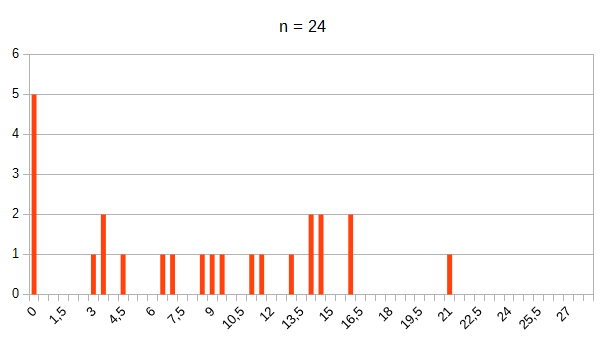
\includegraphics[scale=0.7]{./pics/tut2/statistics-ub2.png}
		%TODO \linebreak \centering $\diameter$ 8,35 bzw. 11,79 von 25 (28)
	\end{frame}
	
	\subsection{3. Übungsblatt - Fehler (Allgemein)}
	\begin{frame}
		\frametitle{Häufige Fehler}
		\begin{block}{Allgemein}
			\begin{itemize}
				\item 			%TODO common faults
			\end{itemize}
		\end{block}
	\end{frame}
	
	\subsection{3. Übungsblatt - Fehler}
	\begin{frame}
		\frametitle{Häufige Fehler}
		\begin{block}{Aufgabe 1 (Plug-In-Architektur): $\diameter$  von 4 (+ 1)} %TODO avg
			\begin{itemize}
				\item %TODO
			\end{itemize}
		\end{block}
	\end{frame}

	\begin{frame}
		\frametitle{Häufige Fehler}
		\begin{block}{Aufgabe 2 (Plug-In): $\diameter$ von 4} %TODO avg
			\begin{itemize}
				\item 	%TODO
			\end{itemize}
		\end{block}
	\end{frame}

	\begin{frame}
		\frametitle{Häufige Fehler}
		\begin{block}{Aufgabe 3 (iMage-Bundle): $\diameter$  von 2} %TODO avg
			\begin{itemize}
				\item 	%TODO
			\end{itemize}
		\end{block}
	\end{frame}

	\begin{frame}
		\frametitle{Häufige Fehler}
		\begin{block}{Aufgabe 4 (Aktivitätsdiagramme (Geometrify)): $\diameter$ von 10} %TODO avg
			\begin{itemize}
				\item 	%TODO
			\end{itemize}
		\end{block}
	\end{frame}

	\begin{frame}
		\frametitle{Häufige Fehler}
		\begin{block}{Aufgabe 5 (Sequenzdiagramm (main-Methode)): $\diameter$ von 5} %TODO avg
			\begin{itemize}
				\item %TODO
			\end{itemize}
		\end{block}
	\end{frame}

	\begin{frame}
		\frametitle{Häufige Fehler}
		\begin{block}{Aufgabe 6 (Substitutionsprinzip): $\diameter$ von 3} %TODO avg
			\begin{itemize}
				\item 	%TODO
			\end{itemize}
		\end{block}
	\end{frame}



\section{Motivation}
	\subsection{Kontext}
		\begin{frame}
			\frametitle{Wo sind wir?}
			\begin{itemize}
				\item die ersten 2 Phasen des Wasserfallmodells sind geschafft
				\pause
				\linebreak $\implies$ Welche waren das nochmal? \pause Planung, Definition!
				\pause
				\linebreak $\implies$ Dokumente? \pause Lastenheft, Pflichtenheft (+ andere\dots)
				\pause
				\item  jetzt: Entwurf!
			\end{itemize}
		\end{frame}
	
		\begin{frame}
			\frametitle{Wozu Entwurf?}
			\centering
			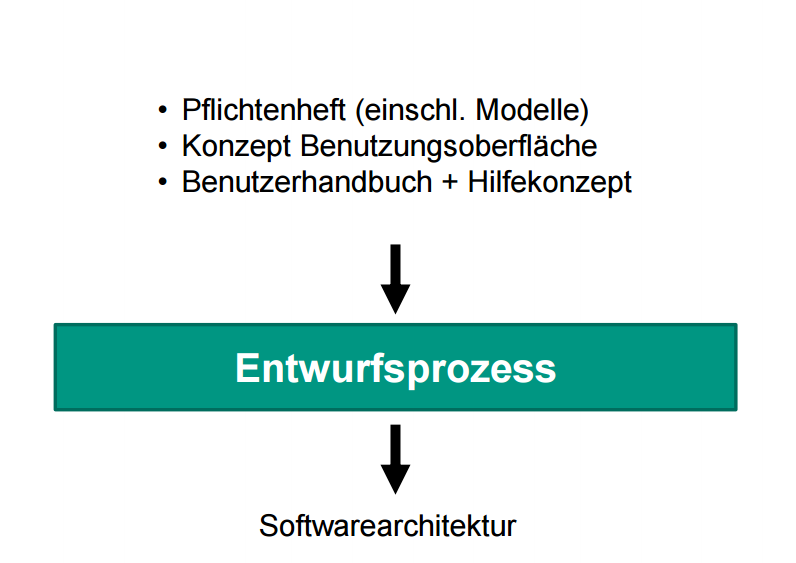
\includegraphics[scale=0.4]{./pics/tut3/design.png} \linebreak
			Softwarearchitektur ist Grundlage für Implementierung!
		\end{frame}
	
		\begin{frame}
			\frametitle{Abgrenzung Definition vs. Entwurf}
			\begin{itemize}
				\item Definition: \textbf{Was} ist zu implementieren?
				\pause
				\item Entwurf: \textbf{Wie} ist das System zu implementieren?
			\end{itemize}
		\end{frame}
	
\section{Entwurfsmuster}
	\subsection{Grundlagen}
	
	\begin{frame}
		\frametitle{Empfehlenswerte Literatur (wirklich!)}
		knapp 700 Seiten \linebreak $\implies$ als interaktives Nachschlagewerk, falls man bestimmte Muster nicht versteht \linebreak
		\centering
		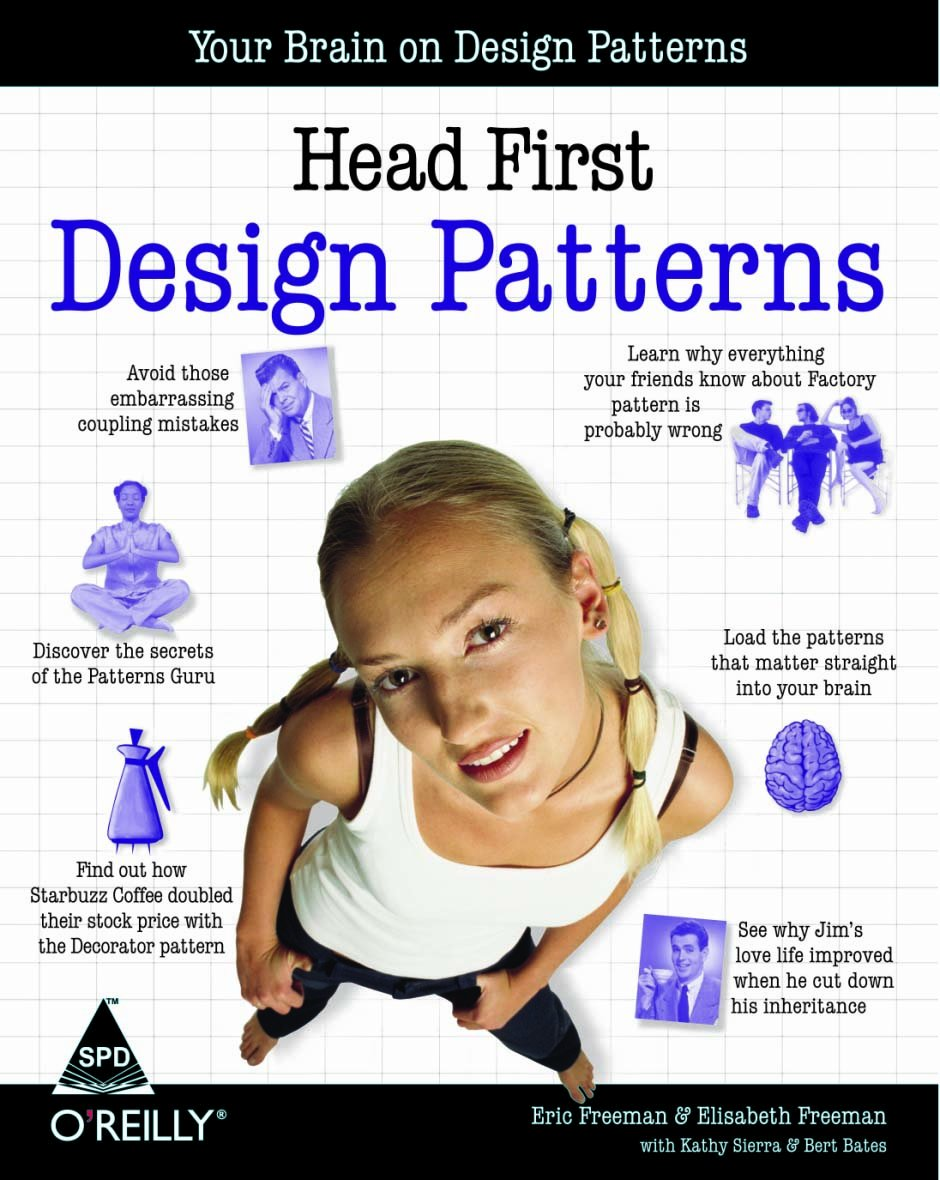
\includegraphics[scale=0.15]{./pics/tut3/literature.jpg}
	\end{frame}
		
	\begin{frame}
		\frametitle{Wozu Entwurfsmuster?}
		\begin{block}{Entwurfsmuster}
			Ein Software-Entwurfsmuster beschreibt eine
			Familie von Lösungen für ein Software-Entwurfsproblem.
		\end{block}
		\pause
		\begin{itemize}
			\item schematische Klassendiagramme zur Lösung von häufig auftretenden Problemen \pause
			\item Wiederverwendung von Entwurfswissen $\implies$ Rad nicht neu erfinden!
		\end{itemize}
		\pause
		\centering
		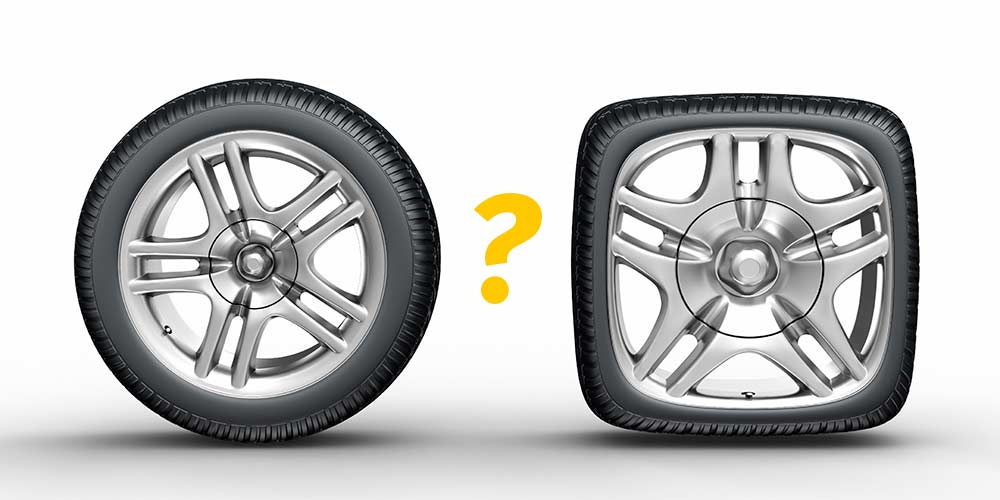
\includegraphics[scale=0.2]{./pics/tut3/new-wheel.jpg}
	\end{frame}
	
	\begin{frame}
		\frametitle{Geheimnisprinzip}
		\begin{block}{Geheimnis- / Kapselungsprinzip}
			Jedes Modul verbirgt eine wichtige
			Entwurfsentscheidung hinter einer
			wohldefinierten Schnittstelle, die sich bei einer
			Änderung der Entscheidung nicht mit ändert.
		\end{block}
		\pause
		Sinn? \pause $\implies$ Änderungen ohne Risiko durchführen \linebreak \pause
		Beispiel? \pause $\implies$ private Attribute mit get()- und set()-Methoden
	\end{frame}

	\begin{frame}
		\frametitle{Vorgriff: Entwurfsmuster Strategie}
		\begin{itemize}
			\item Ziel: Algorithmen kapseln, austauschbar machen
			\item wird in vielen Entwurfsmustern verwendet
		\end{itemize}
		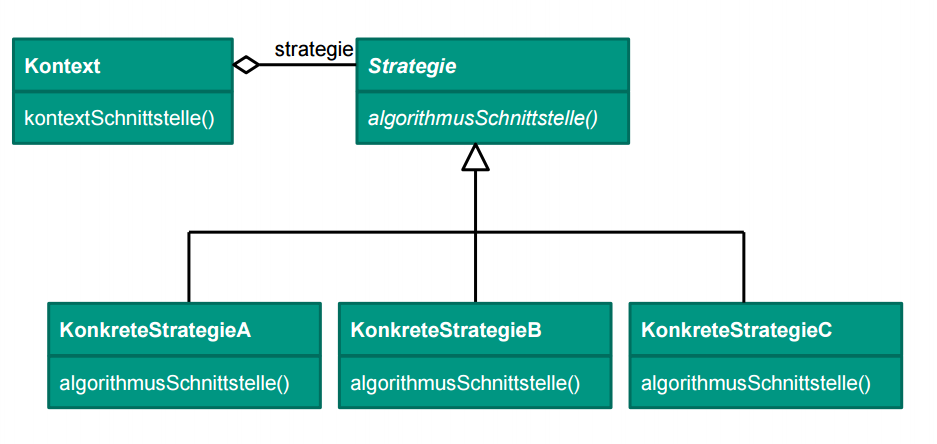
\includegraphics[scale=0.5]{./pics/tut3/strat.png}
	\end{frame}

	\begin{frame}
		\frametitle{Kategorien der Entwurfsmuster}
		\begin{itemize}
			\item \textbf{Entkopplungs-Muster}
				\begin{itemize}
					\item \textbf{Adapter}
					\item \textbf{Beobachter}
					\item \textbf{Iterator}
					\item \textbf{Stellvertreter}
					\item \textbf{Vermittler}
					\item Brücke
				\end{itemize}
			\item Varianten-Muster
			\item Zustandshandhabungs-Muster
			\item Steuerungs-Muster
			\item Bequemlichkeits-Muster
		\end{itemize}
	\end{frame}

\section{Adapter}
	\begin{frame}
		Inhalt...
	\end{frame}

	\section{Beobachter}
	\begin{frame}
	Inhalt...
	\end{frame}

\section{Iterator}
	\begin{frame}
	Inhalt...
	\end{frame}

\section{Stellvertreter}
	\begin{frame}
	Inhalt...
	\end{frame}

\section{Vermittler}
	\begin{frame}
	Inhalt...
	\end{frame}



\section{Tipps}
	\subsection{Tipps}
	\begin{frame}
		\frametitle{Tipps - 4. Übungsblatt}
			\begin{exampleblock}{Aufgabe}
				\begin{itemize}
					\item 	%TODO
				\end{itemize}
			\end{exampleblock}
			\pause
			\begin{exampleblock}{Aufgabe}
				\begin{itemize}
					\item %TODO
				\end{itemize}
			\end{exampleblock}
	\end{frame}

	\begin{frame}
		\frametitle{Tipps - 4. Übungsblatt}
			\begin{exampleblock}{Aufgabe}
				\begin{itemize}
					\item %TODO
				\end{itemize}
			\end{exampleblock}
			\pause
			\begin{exampleblock}{Aufgabe}
				\begin{itemize}
					\item 	%TODO
				\end{itemize}
			\end{exampleblock}
	\end{frame}
	
	\subsection{Abgabe}
	\begin{frame}
		\frametitle{Denkt dran!}
		\begin{alertblock}{Abgabe}
			\begin{itemize}
				\item Deadline am 21.6 um 12:00 %TODO check when released
				%TODO more to remember?
			\end{itemize}
		\end{alertblock}
	\end{frame}
		
	\begin{frame}
		\frametitle{Bis dann! (dann  := 26.06.17)}
		\centering
		%TODO choose comic 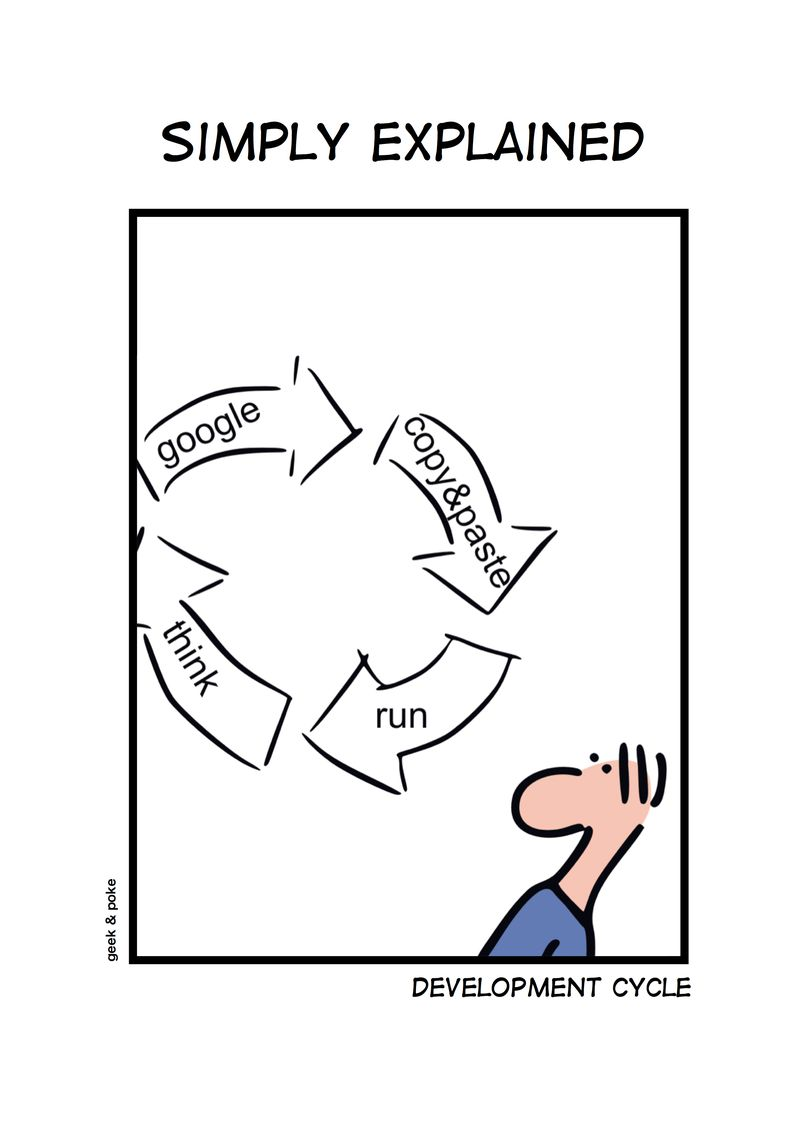
\includegraphics[scale=0.9]{./comics/geek_and_poke_development.jpg}
	\end{frame}

\end{document}